% !TeX spellcheck = hu_HU
% !TeX encoding = UTF-8
% !TeX program = xelatex
%----------------------------------------------------------------------------
\subsection{Átfogó architektúra}\label{subsec:c4:impl:arch}
%----------------------------------------------------------------------------

A C4 fordító és kiértékelő programok a kód nagy részében azonosak: a különbség, hogy a folyamat végén található program bináris kimenetet generál vagy az LLVM \gls{JIT} lehetőségeit kihasználva direkt módon kezdi el kiértékelni a C4 kódnak megfelelő memóriabeli reprezentációt.

\begin{figure}[htb]
    \centerline{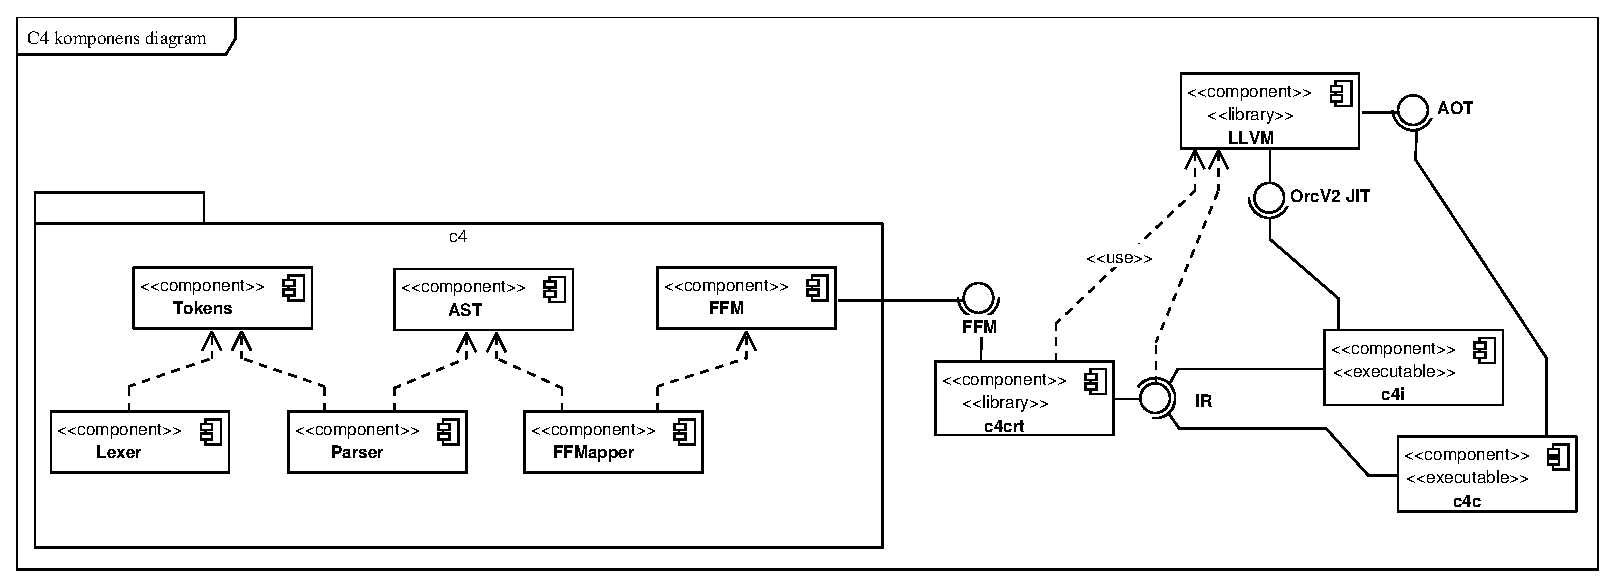
\includegraphics[width=\linewidth]{content/c4-comp.eps}}
    \caption{A C4 projekt architektúra ábrája}\label{fig:c4-comp}
\end{figure}

A feldolgozás az általános fordítói lépéseket tartalmazza: megjelenik a lexikális elemző (lexer), amelyik előállítja a bemenet tokenekké formált változatát és az elemző (parser), amelyik egy absztrakt szintaxis fát (\gls{AST}) állít elő.\footnote{A C4 fordítás közben nem készül külön elemzési fának (parse tree) nevezett szerkezet, amelyik minden szintaktikai elemet tárolna; a fölösleges tokenek azonnal eldobásra kerülnek.}

Az elemző lépés után azonban van egy sajátos lépés, még mielőtt LLVM belső reprezentáció (\gls{IR}) készülne belőle.
Ez egy alacsony szintű, de számítógép architektúra független leírás, amelyet az LLVM biztosít.
Az említett extra lépés látszik \aref{fig:c4-comp}.~ábrán is: ez az a réteg, amelyiket egyszintű függvény-hozzárendelésnek (\gls{FFM}) hívok.
Az LLVM \gls{IR}-nak és a saját \gls{FFM}-nek részletesebb tárgyalása megtalálható \aref{sinsubsec:c4:impl:steps:ffm}.~és \aref{sinsubsec:c4:impl:steps:ir}.~szekciókban.

Az előző bekezdések tartalma mind a {\tt c4} könyvtáron belül történik meg. 
Ennek kimenete egy forrásfájl feldolgozásakor az előbb említett \gls{FFM} struktúrájú leírása a bemenetnek.
Ez lehetővé teszi, hogy a legbelső, általánosan csak a bementi szöveg feldolgozásával foglalkozó könyvtár az LLVM könyvtáraitól független maradjon és könnyebben és gyorsabban fordítható legyen.

A következő lépésben a {\tt c4crt} (C4 fordító futtató környezet, C4 Compiler Runtime) könyvtár felhasználja a {\tt c4} által előállított \gls{FFM} formátumú leírást, és az LLVM számára feldolgozható LLVM \gls{IR}-t elkészíti belőle.

A folyamat végén pedig vagy a {\tt c4c} vagy {\tt c4i} bináris áll, a felhasználó végcéljától függően.
Ezek az előző lépésben előállított LLVM \gls{IR}-t a megfelelő LLVM alkönyvtár számára továbbítják: a fordító olyan binárist generál belőle, amelyet natívan lehetséges futtatni, a kiértékelő pedig helyben végrehajtja azt, igény szerinti fordítással (\gls{JIT}).
Az optimalizálás lépése is ezekben a lépésekben történik meg, már az LLVM \gls{IR}-on.

\subsection{A C4 fordító lépései}\label{subsec:c4:impl:steps}

\subsubsection{Lexikális elemző}

A lexikális elemző elég általános, nem tartalmaz kifejezetten érdekes megvalósításokat.
Minden token egy külön osztályba kerül, amelyek fordítási idejű konstans kifejezések ({\tt constexpr}) formájában tárolják, hogy milyen literális szöveget vagy \gls{PCRE} kompatibilis reguláris kifejezést kell hozzá illeszteni.
A megadott érték alapján fordításkor dönti el a rendszer, hogy melyiket használja hozzá.
A token által hivatkozott szöveg mindig a memóriába lapozott (memory mapped) forrásfájl egy részére mutat, így a tokenek soha nem foglalnak extra memóriát.
A lexikai elemző osztály kérésenként egyesével egy összegtípusban (sum type, {\tt std::variant<...>}) adja vissza a mindenkori következő tokent.

\subsubsection{Elemző}

Az elemző egy kézzel írt megvalósítása a rekurzív leereszkedő elemző (recursive descent parser) algoritmusnak; a kód a legtöbb helyen így ezzel megfelelően pár függvény, amelyik rekurzívan hívják egymást.
Két dolog azonban figyelmet érdemel: a függvényhívások és a felhasználó által bevezetett operátorok kezelése.

Az következők előtt megjegyzésre méltó, hogy a névfeloldás elemzés közben megtörténik, nem kell külön lépést bevezetni rá.
Ez a nyelv felépítésének következménye: minden függvény paraméterezését (paramétereinek számát, mivel dinamikus típusozás van) ismerni kell hívása előtt.
Emiatt azonban minden függvény be van jegyezve a fordító által ismert függvények közé, így mire meghívódik egyből fel is lehet oldani a megfelelő belső függvény leíró adatszerkezetre való mutatóval.

Mivel a C4 nyelv szintaxisában gyakorlatilag a szóköz a függvényhívás szintaktikája, így a függvények hívásakor egy speciális esetet kezelni kell: a hívott függvény alapján meg kell keresni, hogy mennyi paraméter tartozik hozzá és annyi darab kifejezést kell a argumentumként keresni, vagy hibát jelezni ennek hiányáról.

Az elemzőkben az operátorokat általánosan is extra figyelemmel kel kezelni: a különböző precedencia szinteket és az asszociativitást vagy már az elemzés közben figyelembe kell venni, vagy egy külön utófeldolgozási lépésben kell helyreállítani a megfelelő hívási sorrendet az operátorokból.
Emiatt elemző generátor eszközök használatánál (\pl Bison, Xtext) a különböző precedenciákat a rekurzió különböző szintjeire való elhelyezésével szokás megoldani a szabályok megadásakor.
Kézzel fejlesztett megvalósítások esetén azonban egy hatékonyabb lehetőségünk is van, az \un precedencia mászó algoritmus (precedence climbing algorithm) formájában.
Az eredeti algoritmust a BCPL-ről írt könyvben definiálták BCPL-ben és szöveges formában \cite{richardsBasicCombinedProgramming1984}, de egy verziója elérhető példakóddal az ANTLR3 eszközhöz is \cite{harwellOperatorPrecedenceParser2008}.
Ennek a manuális megvalósításával hatékonyan lehetséges általánosan infix formájú operatorokat elemezni.
Annyi módosításra van szükség, hogy a konstans halmazt, amelyikkel a lehetséges operátorokat definiálják, egy elemzési időben változó halmazra kell cserélni.

Ezt az algoritmust felhasználva az említett módosítással bármely felhasználó által definiált asszociativitású és precedenciájú operátort tartalmazó kifejezést lehetséges helyesen \gls{AST}-be konvertálni, külön utófeldolgozás nélkül.

Az elemzési folyamatnak a ki- és bemenetét mutatja be \aref{fig:c4-ast}.~ábra.
Ezen az ábrán a {\tt ->}, {\tt @} és {\tt \#} után álló mutatók értékei egyszerűsítve lettek utolsó két karakterükre a {\tt c4c} \gls{AST}-t lekérdező kimenetében, hogy könnyebben olvasható legyen az ábra.
Ezek értelmezése a következő: {\tt \#} egy paramétert vezet be, a {\tt @} pedig egy függvényt.
Az utánuk található mutató érték a jelenlegi futás során, a fordító által használt belső objektum memóriacíme. 
A visszamaradó {\tt ->} jelzi, hogy melyik memóriacímen helyezkedik el az, amit a név alapján hivatkozik; ha nincs mögötte cím (pl. {\tt +/2->}), akkor egy beépített függvényről van szó, amelyik feloldása majd az \gls{FFM} fázisban történik meg. 
A {\tt scope} elemek feladata, hogy számon tartsák a külső függvényekből hivatkozott szimbólumokat. 
Ez a következő lépéseknél, ahol explicitté válnak a lezárások tárolt értékei, a számítások gyorsítását teszi lehetővé.

\begin{figure}
    \centerline{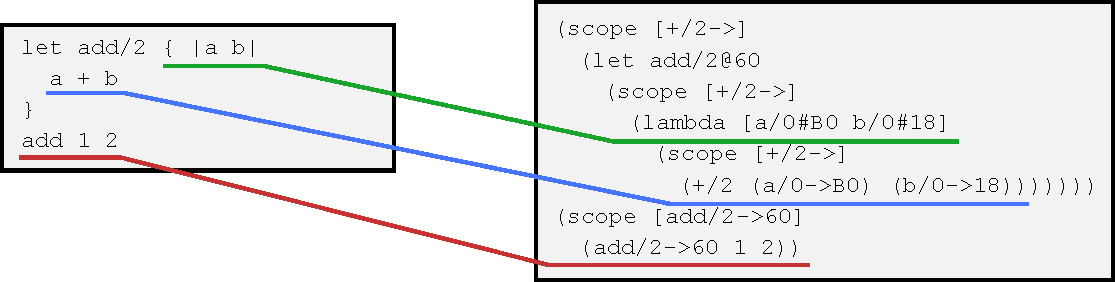
\includegraphics[width=.8\linewidth]{figures/ast.pdf}}
    \caption{A C4 forrásból készített AST (mutató értékek egyszerűsítve)}\label{fig:c4-ast}
\end{figure}

\subsubsection{Egyszintű függvény-hozzárendelő}\label{sinsubsec:c4:impl:steps:ffm}

A következő lépés az egyszintű függvény hozzárendelés.
Ez egy olyan köztes lépés, amelyik a megvalósítást teszi könnyebbé.
A következő lépés kimenete (LLVM \gls{IR}), és ennek a lépésnek a bemenete (\gls{AST}) között akkora különbség van szemantikailag, hogy a megvalósító kód olvashatóságának és karbantarthatóságának rovására menne rögtön egy lépésben leírni ezt a transzformációt.
Ez az eltérés könnyen látszik: az \gls{AST}-ben leírt nyelv egy lusta kiértékelésű, dinamikusan típusos, immutábilis nyelv,  az LLVM \gls{IR} pedig egy regiszterek szintjén működő, gép független assembler nyelv.

Az \gls{FFM} réteg ezt a problémát egyszerűen úgy oldja meg, hogy sok olyan implicit elemet, ami az eredeti C4 nyelvben és így az \gls{AST}-ben sem jelenik meg külön, azt egy \gls{FFM} szinten explicit jelölt nyelvi elembe emeli ki.

Feltűnő eltérés a függvényhívások két fajtája: egy blokk legfelső szintjén azok a hívások, amelyek direkt a kapcsos zárójelek között vannak, és azok amelyek más függvények paramétereként állnak. 
Előbbiek átlagos szorgos (eager) kiértékeléssel futnak le, így ezeket egyszerű {\tt call} elemekbe kell átfordítani.
Utóbbiak az \gls{FFM} szinten a lusta {\tt pack} hívással vannak reprezentálva.
Ez a csomagolás nevezéktan a későbbi lépésekben generált segédfüggvényekben is megjelenik, amelyek a futtatókörnyezet {\tt c4rt\_package\_t} típusát használják egy-egy ilyen függvényhívás végrehajtására.

Az \gls{FFM} névadó lépéséről viszont még nem esett szó.
Minden blokk a C4 nyelvi szinten egy különálló függvényként viselkedik: lehetnek paraméterei, van valamekkora törzse amelyik kiértékelésekor visszaad valamilyen értéket.
Viszont a fordítás végére a bemenetből egy LLVM \gls{IR} formátumú kimenetet kell előállítani, amelyik nem támogat egymásba ágyazott függvény definíciókat.
Így az összes blokk egymásba ágyazást ki kell bontani, és a globális függvények szintjére hozni.

Ehhez szükség van valamilyen névátalakítás (mangling) műveletre:
minden blokknak a programon belül globálisan egyedi nevet kell adni, az anonim blokkok és blokkokon belül definiált függvények miatt viszont ez nem teljesül automatikusan.
Ennek a konkrét részleteire most nem térek ki, mert nem kifejezetten érdekes.
A lényegi lépések nagy vonalakban: 1) minden anonim blokk a direkt beágyazó blokkon belüli sorszámát kapja meg névnek; 2) a generált teljes névben a blokk saját nevét megelőzi minden ősének a neve beágyazási sorrendben; 3) az operátorok az angol ábécé karaktereit tartalmazó függvényneveket kapnak (\pl {\tt +} \textrightarrow {\tt p}).
Az operátoroknál kiemelendő, hogy az operátorok {\tt \_Co}-val, az egyszerű függvények {\tt \_Cs}-el kezdődnek, így nem okoznak egymás között névütközést.

Adódik azonban még egy probléma az egyszintű függvények létrehozásával.
Egy blokkon belül definiált blokk C4-ben egyszerűen, extra jelölés nélkül tud hivatkozni a külső függvényekre vagy paraméterekre.
Viszont minden függvényt egy globális szintre kell felhozni, így ezeket az implicit hivatkozásokat a függvények törzsében fel kell oldani egy érvényes memóriacímből való olvasásra.
Azokat a függvényeket, amelyeket ilyen módon át kell alakítani lezárásnak (closure, és innentől az angol nevét használom) hívják.
Speciális tulajdonságuk, hogy a viselkedésük függővé válik a létrejöttük pillanatában érvényes változók értékeitől.
Ezt mutatja be \aref{lst:closure-bhv}.~listázásban található kódrészlet: a closure viselkedése megváltozik az {\tt a} paraméter értékétől.

\begin{lstlisting}[gobble=4,label=lst:closure-bhv,caption={A closure viselkedés bemutatása}]
    let mk_closure { |a|
        { a + 1 } # <- ez a blokk a closure
    }

    # &(...)/N egy kifezejzében értékként tárolt függvény hívása
    println &(mk_closure 40)/0 # => 41
    println &(mk_closure 41)/0 # => 42
\end{lstlisting}

Az utolsó megoldandó probléma az a belépési pontja a programnak.
A C és hozzá hasonló nyelvekben a program futásának kezdete egy függvény formájában van definiálva.
Például C-ben ezt a szerepet a globális {\tt main} függvény tölti be.
Vannak nyelvek azonban, mint \pl Perl, Ruby és Python, amelyek ezt nem definiálják, hanem a programként adott fájl sorban kezd el futni, külön belépési függvény nélkül.
Ez általában a rugalmasabb, dinamikusan típusos nyelvekre jellemző, és a C4 is ebbe a kategóriába tartozik.
Az LLVM \gls{IR} azonban a belépési függvény definíciójánál is alacsonyabb szintű.
A program futásának kezdetét az operációs rendszer által meghatározott módon kell kezelni.
C nyelv fordítói ezt az operációs rendszer függő problémát a megfelelő C könyvtárban valósítják meg.
Ezzel párhuzamban egy hasonló megvalósítást adok a C4 fordítás esetében is: az a kód, amelyik nem tartozik semmilyen függvényhez, az az \gls{FFM} rétegben egy {\tt \_C@main} függvény törzsébe kerül generálásra.
A bináris generálásnál pedig a platformnak megfelelő belépési ponton keresztül meghívja ezt a függvényt.
A szimbólum neve garantálja, hogy nem lesz névütközés C4-ben definiált függvényekkel, LLVM pedig tudja kezelni ezt a különleges azonosítót.

Ezeket a lépéseket és megoldásokat használva előáll az \gls{FFM} réteg végén egy \gls{FFM} formátumú leírása a bemeneti C4 forrásból előállított \gls{AST}-nek.
Ennek a transzformációnak az eredménye \aref{fig:c4-ffm}.~ábrán látható.
Ezen az ábrán nagyszerűen látszik az is, hogy a C4 a függvényeket és operátorokat teljesen egyformán kezeli a elemzési lépés után.
A deklarációk a kódrészlet elején az összes használt függvény számára megjelennek, ezek a {\tt decl}-el kezdődő sorok. 
Ezt követik a megvalósítással rendelkező függvények definíciója ({\tt defn}): 
a beépített megvalósítású {\tt +/2} operátor ({\tt \_Co1p2E}) látható, hogy csak deklarálva van. 
Ezek megegyeznek a későbbiekben az LLVM \gls{IR}-be generált deklarációkkal és definíciókkal.

\begin{figure}[htb]
    \centerline{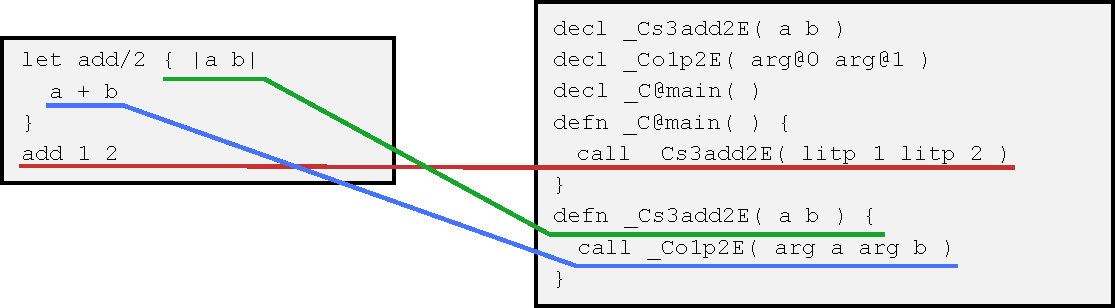
\includegraphics[width=.8\linewidth]{figures/ffm.pdf}}
    \caption{A C4 forrásból készített FFM}\label{fig:c4-ffm}
\end{figure}

\subsubsection{\gls{IR} előállítása és kimenet generálása}\label{sinsubsec:c4:impl:steps:ir}

Az utolsó lépésben kerül előállításra az előzőekben már említett LLVM \gls{IR} leírása az eredeti C4 kódnak.
Ez egy olyan formátuma az LLVM rendszernek, amelyiket bemenetként várnak a különböző alrendszerek.
Ez szolgál egy olyan rétegként, amelyik elég általános ahhoz, hogy ne kötődjön egy konkrét hardverhez sem túlságosan, de elég alacsony szintű ahhoz, hogy a lehető legtöbb olyan koncepciót, amivel egy-egy platform assembly nyelve rendelkezik, képes legyen megfelelő pontossággal kifejezni.

Az LLVM \gls{IR} egy úgy nevezett statikus egyszeri értékadás (\gls{SSA}) formát használ, amelyikben minden regiszter pontosan egyszer állhat értékadás bal oldalán.
(A regiszterek száma nem korlátozott.)
Az ennek a feltételnek megfelelő utasítások sorát pedig egy-egy felbonthatatlan egységként\footnote{Félreértéseket elkerülendő, a párhuzamosítási kontextusban is használt ,,atomi'' kifejezés használatát kerülöm. Párhuzamos kiértékelés esetén egy egyszerű blokk lefutása nem garantáltan atomi, de az még akkor is garantált, hogy ha belépünk egybe, akkor annak minden utasítását végrehajtjuk.} lefutó egyszerű blokkba (basic block) kell rendezni, amelyek között (feltételes) ugrásokkal lehet váltani a blokk végén.
Olyan esetekben, ahol egy regiszter értéke valamilyen futásidejű döntéstől függ, mondjuk egy if két ágán másképpen alakul annak tartalma, az elágazás után ezt újra össze kell vonni, különben nem lesz egy  olyan statikusan megállapítható regiszter,  amelyik biztosan a megfelelő értéket tartalmazza.
Erre ad megoldást a $\phi$ függvény: olyan egyszerű blokkok elején helyezkedhet el, ahol két ilyen módon különböző regisztert kell egybe fésülni.
Működése egyszerű: a bemenetén szereplő regiszterek közül az kerül felhasználásra, amelyik abból az egyszerű blokkból származik, amelyikből beléptünk a jelenlegibe. 
Ez a megfelelő hardveres ekvivalens értékadássá alakul át kódgeneráláskor.

Ha ezeket a blokkokat felrajzoljuk egy gráf csúcsainak, majd az ugrások irányával azonos irányba behúzunk éleket, akkor egy \un vezérlésfolyamgráfot (\gls{CFG}) kapunk, amivel a függvények teljes törzsét írjuk le.
Egy ilyen \gls{SSA} transzformációra látható egy egyszerű példa \aref{fig:ssa-tr}.~ábrán. 
Az ábrán található $\phi$ függvény a színkódolásnak megfelelően viselkedik:
ha a kék nyílnak megfelelő egyszerű blokkból érkezünk az
,,if.after'' blokkba, akkor a kék pontozott vonal szerinti változót adja értékül. 
Ezzel analóg a viselkedés a zöld nyíl esetén.

\begin{figure}[htb]
    \centering
    \begin{subfigure}{.2\linewidth}
        \begin{lstlisting}[gobble=12,numbers=left]
            a = 1
            if c > 0
              a = 2
            print a
        \end{lstlisting}
        \caption{Pszeudokód}
    \end{subfigure}
    \begin{subfigure}{.6\linewidth}
        \centerline{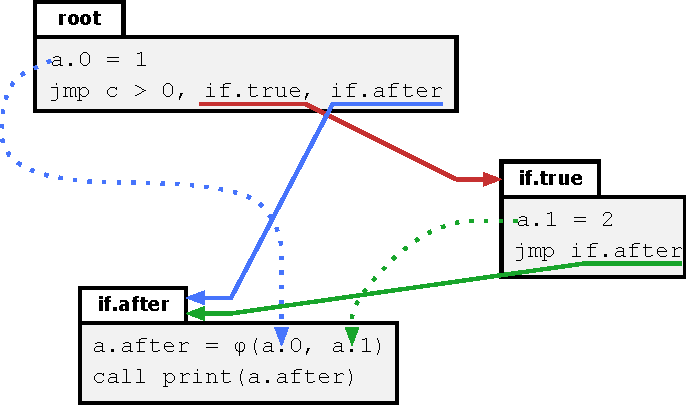
\includegraphics[width=.95\linewidth]{figures/ssa.pdf}}
        \caption{\gls{SSA} átírás egyszerű blokkokkal egy \gls{CFG}-be}
    \end{subfigure}
    \caption{Pszeudokód példa átírása \gls{SSA} formába}\label{fig:ssa-tr}
\end{figure}

Ennek a sémának az elsődleges előnye a fordításkor használt optimalizáló és a hozzá fejlesztett egyes optimalizációs lépések megvalósításában jelenik meg.
Az \gls{SSA} forma miatt ezek sokkal könnyebben kivitelezhetőek, mert minden regiszter értéke egyértelműen ismert az egyetlen értékadásból, amelyikben bal oldalt szerepel.
Ez alapján pedig könnyebben lehet különféle következtetéseket levonni, információt gyűjteni a kód viselkedéséről, ami alapján pedig a kód formáját átírni, hogy az jobban közelítse az optimálisat.
Mivel ez a séma nagyon elterjedt a fordító backendekben, az optimalizációs lépésekből létezik számos akadémiai -- például a $\phi$ függvények hatékonyabb elhelyezésével foglalkozó \cite{boissinotRevisitingOutofSSATranslation2008} -- és a gyakorlatban megvalósítottakból is megannyi implementáció létezik.
Nagy számban megtalálhatóak ilyenek az LLVM kódbázisában a saját \gls{IR} formátumán futtatható módon.

Összességében, az LLVM használatához át kell alakítani a bemeneti forrásnyelv leírását \gls{SSA} formába.
Erre a feladatra már a kilencvenes éveke eleje óta létezik algoritmus \cite{cytronEfficientlyComputingStatic1991} és annak különféle javításai \cite{briggsPracticalImprovementsConstruction1998}.
Röviden kifejtve azonban az \gls{IR} generálásának szempontjából két nagy következménye van.
Első, hogy ha egy forrásnyelvi változó többször kap értéket egy program folyama során, akkor azt olyan módon kell \gls{SSA} formába hozni, hogy minden értékadásnál egy új verziót kell hozzá bevezetni egy regiszter formájában.
A \gls{CFG} és érintett $\phi$ függvények szerinti jelenleg megfelelő verziót pedig számon kell tartani, és a változóra vonatkozó hivatkozásokat a legutolsó regiszter példányra kell feloldani.
A másik, hogy egy elágazó \gls{CFG} esetén a $\phi$ függvényeket megfelelő paraméterezéssel le kell generálni minden olyan blokk elejére, amelyikbe több beérkező él is van.

Az \gls{SSA} generálás következményeit azért fejtettem ki, mert a C4 megvalósításban az általános algoritmusnál egyszerűbb megoldást lehetséges adni.
Az első következmény nem játszik szerepet, hiszen minden immutábilis a forrásnyelvben is, így nem kell ezzel külön foglalkozni, automatikusan megfelel az \gls{SSA} elvárásainak.
Ami viszont érdekesebb, hogy a másodikkal sem kell foglalkozni, mert nincs külön elágazás vagy ciklus eleme a nyelvnek, ami nehézségeket okozna.
Az {\tt if/3} például is csak egy olyan függvény, mint \aref{fig:c4-ffm}.~ábrán definiált {\tt add/2}.
Meghívása pedig emiatt teljesen azonos, és így nincs elágazás.
Ezeknek megfelelően az \gls{IR} generálásánál csak az egyes struktúrákba való indexelést (lusta paraméterátadás struktúráinál) és a lusta függvényhívást kell legenerálni a primitívebb ekvivalenseikbe.
Ezek már nem kifejezetten nehéz feladatok, mivel segédfüggvényként lehetséges bevonni olyan kódrészleteket, amelyeket már előre és egyszer megvalósítottam, kézzel.
A segédfüggvények feladatköre \aref{sec:c4:rt}.~szekcióban tárgyalt viselkedések megvalósítása.

Kérdéses lehet az előző bekezdésben adott azon állítás, hogy nincs elágazás generálása szükség: ha egyáltalán nincs elágazás, akkor hogyan lehetséges megvalósítani azt, hogy a nyelvben mégis elérhető és használható az {\tt if/3} függvény?
A C4 képes arra, hogy olyan módon definiáljon igaz és hamis értékeket, majd ezek felett egy elágazás szerkezetet, hogy az a más nyelvekből megszokott szintaktikájú és szemantikájú {\tt if} szerkezetre hasonlítson.

Ennek a megmagyarázáshoz előbb röviden be kell vezetni a $\lambda$-kalkulust \cite{churchSetPostulatesFoundation1932}.
Ez egy olyan matematikai modellje a számításnak, amely azonos kifejezőerejű a Turing-gépekkel \cite{turingComputabilityLdefinability1937}.
Három elemi komponensből áll: változókból, $\lambda$ absztrakciókból és alkalmazásból (application).
Utóbbi kettőt érdemes kifejteni. 
Egy $\lambda$ absztrakció egy olyan kifejezés, amelyik bevezet egy bemeneti változót kötött formában. 
Formája: $\lambda x.\mathcal{F}(x)$, ahol $\mathcal{F}$ egy olyan kifejezés, amelyben az $x$ változó kötetlen formában szerepelhet.
Egy alkalmazás pedig egyszerűen egy olyan $s\;t$ kifejezés, amelyben $s$ és $t$ kifejezések.

A számítás végrehajtására a $\beta$-redukció szolgál, amelyben egy $s\;t$ alkalmazás esetén, az $s$ legfelső szinten kötött változójának minden előfordulását behelyettesítjük $t$-vel.
Ennek a felhasználásával különböző kiértékelési sorrendeket lehet definiálni, amelyek a rövid bevezetésen túlmutatnak \cite{Sestoft2002}.

A $\lambda$-kalkulusban definiált Church-boolean \cite[2.4.2.~szekció]{kempTheoreticalFoundationsPractical2007} kódolást fel lehet használni az igaz és hamis logikai értékek definiálásra, majd olyan logikai függvényeket, mint az ÉS és a VAGY lehet megvalósítani ezeket felhasználva.
A megvalósítás maga egyszerű:
viselkedésüket tekintve az ,,igaz'' és ,,hamis'' értékek két paraméteres $\lambda$-absztrakciók: 
az igaz az első a hamis a második paraméterét adja értékül. 
A C4 implementáció esetén még külön ki kell értékelni a megfelelő paramétert. 
Ez a nyelv működése miatt van, mert $\lambda$-kalkulussal ellentétben, nem egy külső folyamat ($\beta$-redukció) adja meg a kiértékelést és annak sorrendjét, hanem a nyelvben adott függvények. 
Amint definiálva vannak, ezek használhatóak C4-ben úgy, mint más nyelvek beépített ,,{\tt true}'' és ,,{\tt false}'' literálisai.

Az így adott logikai rendszerben megadható függvények közé tartozik egy olyan elágazás is, amelyik az első bemenetének értéke alapján vagy a második vagy a harmadik bemenetét adja vissza értékül.
Ez pontosan az az if konstrukció, amelyiket függvényként lehet használni, többek között C4-ben is.
Ennek a megadása látható \aref{fig:churh-bools}.~ábrán, ahol az ekvivalens C4 kóddal együtt szerepel.

\begin{figure}[htb]
    \begin{subfigure}{.45\linewidth}
        \begin{align*}
            \mathrm{true}  &\triangleq \lambda t.\lambda f.t \\
            \mathrm{false} &\triangleq \lambda t.\lambda f.f \\
            \mathrm{if}    &\triangleq \lambda c.\lambda t. \lambda f.c\;t\;f \\
            \mathrm{if}\ \mathrm{true}&\;\mathrm{false}\;\mathrm{true} \overset{\beta}{\rightsquigarrow}  \mathrm{false}
        \end{align*}
    \end{subfigure}
    \begin{subfigure}{.45\linewidth}
        \begin{lstlisting}[gobble=12,numbers=left]
            # Hogy elkerüljem a beépített függvényekkel
            # való névütközést c-vel vannak prefixelve
            let ctrue { { |t f| &(t)/0 } }
            let cfalse { { |t f| &(f)/0 } }
            let cif/3 { |c t f| &(c)/2 t f }

            cif ctrue
                println "true"
                println "false" # => true
        \end{lstlisting}
    \end{subfigure}
    \caption{A Church-booleanok $\lambda$-kalkulusban és C4-ben}\label{fig:churh-bools}
\end{figure}

A tényleges megvalósítás azonban mégsem ezt a megoldást használja, mivel így minden elágazás esetén két indirekt címre való ugrást kell végezni végrehajtás közben.
Egyet, amikor a beérkező feltétel paraméterben lévő blokkot értékeljük ki, majd amikor ez a blokk továbbugrik a szintén paraméterében kapott igaz vagy hamis blokkot reprezentáló értékre.
Ellenben, ha ezt direkt módon LLVM \gls{IR}-ben adom meg, akkor egy indirekt függvény címére kell csak ugrani: a megfelelő igaz vagy hamis blokkéra.
A logikai érték kiértékelését egy egyszerű szám összehasonlítással meg lehet valósítani.
Erről \aref{ssubsec:c4:rt:types:nan}.~részben leírtak alapján van könnyedén lehetőség.

Az elágazás mellett érdekes lehet valamilyen ciklus megvalósítása, hiszen ezek sok nyelvben beépített nyelvi elem formájában jelennek meg.
Érdemes megjegyezni, hogy ezek az elemek kicsit tájidegenként hatnak egy funkcionális, immutábilis nyelvben, így bemutatásuk célja pusztán a nyelv kifejezőerejének ismertetése. 
Ehhez egy egyszerű \hbox{,,while''} ciklus mutatok be, aminek kódja megtalálható \aref{lst:while}.~listázásban. 
Látható, hogy ez egy rekurzív függvény, azonban annak egy speciális \un jobb rekurzív (tail recursive) verziója.
Mivel a blokk utolsó kiértékelt függvénye, ezért a fordító meg tudja tenni, hogy nem egy függvényhívást, hanem egy egyszerű ugrást generál belőle: ez azonban pont egy nagyon
alacsony szintű ciklussá teszi.

\begin{lstlisting}[gobble=2,numbers=left,label=lst:while,caption={Egyszerű ,,while'' ciklus megvalósítása és használata}]
	let while/2 { |cond body|
		if cond {
			&(body)/0
			while cond body # jobb rekurzió
		}
		else { }
	}
	
	println "Szeretne feldolgozni szöveget? (igen/nem)"
	while { readln == "igen" } {
		println "Adjon meg egy sornyi szöveget: "
		println process readln
		println "Szeretne másikat is feldolgozni? (igen/nem)"
	}
\end{lstlisting}









